\section{Introduction}
\label{sec:intro}

With the rapid development of intelligent transportation, autonomous driving, and urban management, digital twin technology, as an important innovative tool, has gradually shown tremendous potential in various fields\cite{Alpher17}. 
A digital twin refers to the creation of a digital model corresponding to the real world through the real-time synchronization of data collected from the physical world and virtual models\cite{Alpher20c}. 
This technology can simulate, analyze, and optimize the real world in a virtual environment, thus providing support for decision-making\cite{Alpher21b}. 
In the field of autonomous driving, digital twin technology can accurately replicate factors such as traffic flow, road structure, and pedestrian behavior, providing a precise testing and training environment for the perception, planning, and control of autonomous driving systems\cite{Alpher24}\cite{Alpher20d}.

The focus of this research is to apply digital twin technology to the development and testing of autonomous driving systems to improve the interpretability and robustness of autonomous driving systems by replicating real traffic flow scenarios\cite{Alpher24b}.
By constructing high-precision digital twin models and combining reinforcement learning with simulation platforms, we are able to simulate complex driving scenarios and train and optimize autonomous driving algorithms\cite{Alpher22c}. 
At the same time, digital twin technology can provide smarter decision support for traffic management, promoting the development of smart city construction\cite{Alpher17b}.

\begin{figure}[t]
	\centering
	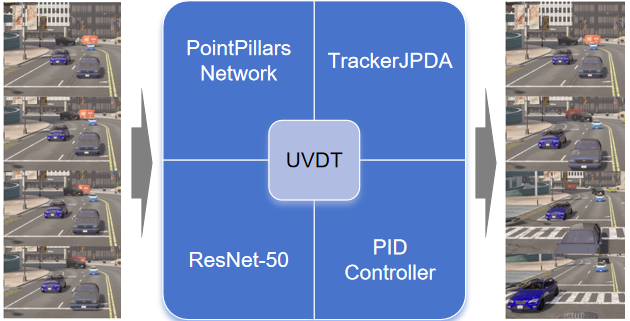
\includegraphics[width=\linewidth]{picture/picture1.png} 
	\caption{Overall Preview of Digital Twin through UVDT} 
	\label{fig:example} 
\end{figure}

We primarily conducted research from four aspects: single-intersection multi-target tracking, multi-intersection multi-target tracking, trajectory inference and restoration, and digital twinning. 
By fusing camera and radar detection, we improved the accuracy of vehicle detection, addressing challenges such as occlusion and perspective changes, thereby optimizing multi-target tracking performance. 
We collected a large amount of training data to train the tracking model, further enhancing tracking performance. 
We inferred trajectories in unknown regions and combined them with the trajectories obtained from multi-target tracking within intersections, ultimately achieving complete trajectories. 
Using the PID control algorithm, we implemented digital twinning by following the previously obtained trajectories.

Vehicle detection is a core perception task in autonomous driving systems, which usually relies on data from various sensors (such as lidar, cameras, and millimeter-wave radar) for object recognition and positioning. As a key input source for digital twin systems, the accuracy of vehicle detection directly affects the behavior modeling and scene restoration quality of traffic participants in virtual environments. 
In recent years, the application of deep learning technologies has significantly improved the accuracy and robustness of vehicle detection. 
On the contrary, through digital twin technology, we can create precise virtual environments to provide abundant training data for autonomous driving systems, enhancing detection performance. 
Digital twins not only improve detection effectiveness in complex and dynamic environments but also optimize the fusion of data from different sensors\cite{Alpher20}.

Object tracking is a key technology in autonomous driving, particularly in multi-object tracking, where the task becomes especially complex due to target occlusions, changes in viewpoint, and misalignment between multiple cameras. 
The accuracy and robustness of object tracking directly affect the credibility of the digital twin system, and its output results (such as target ID consistency and trajectory continuity) can be used to verify the timing consistency of sensor simulation in the virtual environment, detect physical rule deviations in scene modeling, and optimize the motion prediction algorithm of the digital twin.
When the tracking algorithm has ID switching or trajectory breakage in complex scenes, these abnormal data can reveal the potential defects of the digital twin system in terms of dynamic object interaction, multi-sensor synchronization, or environment rendering accuracy, thereby providing data support for the iterative optimization of the simulation model and continuously enhancing the environmental authenticity and behavioral reliability of the digital twin system\cite{Alpher22b}.

Vehicle re-identification (Re-ID) refers to recognizing the same vehicle at different times and locations, especially across multiple viewpoints and different cameras. 
By constructing a vehicle dataset with continuous time series, variable perspectives and dynamically changing environments in a virtual simulation environment, rich feature learning materials are provided for the training of the re-identification algorithm.
The trained algorithm can not only effectively distinguish the skeleton models of different vehicles through precise feature matching, but also accurately identify the color changes of the same vehicle under different lighting conditions, thereby providing a reliable identity association basis for vehicle tracking in multi-camera scenarios, and ensuring the continuity and consistency of vehicle motion trajectories in complex environments\cite{Alpher23}.
This technical path based on virtual data training and real scene verification not only improves the robustness of the re-identification algorithm, but also lays a solid foundation for the precise tracking of intelligent transportation systems.

Trajectory restoration aims to reconstruct complete and continuous vehicle motion trajectories in complex urban road environments through advanced algorithms.
In practical applications, due to the detection distance limitations of multi-target trackers, coupled with interference factors such as target occlusion and sensor noise, tracking interruptions and trajectory breaks often occur.
To meet this challenge, the system needs to combine kinematic models and deep learning algorithms to intelligently infer and complete the lost trajectory fragments to ensure the spatiotemporal continuity of the trajectory.
Finally, by accurately simulating the vehicle's driving route and traffic behavior through integrated control algorithms, a complete autonomous driving system verification platform is formed, providing a reliable digital twin foundation for algorithm development and safety assessment\cite{Alpher24c}.

